\documentclass[12pt, a4paper]{article}

\usepackage[a4paper, top=2.5cm, bottom=2.5cm, left=2.5cm, right=2.5cm]{geometry}
\usepackage{graphicx}
\usepackage{amsmath}
\usepackage{amssymb}
\usepackage{float}
\usepackage{caption}
\usepackage{subcaption}
\usepackage{booktabs}
\usepackage{parskip}
\usepackage{microtype}
\usepackage{siunitx}
\usepackage{enumitem}
\usepackage[hidelinks]{hyperref}
\usepackage{titlesec}
\usepackage{fancyhdr}

% Header/footer
\pagestyle{fancy}
\fancyhf{}
\rhead{42059/41034 --- Lab 2}
\lhead{CMOS Inverter}
\cfoot{\thepage}

% Section formatting
\titleformat{\section}{\large\bfseries}{}{0em}{}[\titlerule]
\titleformat{\subsection}{\normalsize\bfseries}{}{0em}{}

% Image path
\graphicspath{{drive-download-20260305T060328Z-1-001/}}

% Fix for filenames with special characters
\usepackage{grffile}

\begin{document}

%------------------------
%  TITLE PAGE
%------------------------
\begin{titlepage}
    \centering
    \vspace*{1.5cm}

    {\LARGE\bfseries 42059 / 41034\par}
    {\LARGE\bfseries Electronic Components and Fabrication\par}
    \vspace{0.8cm}
    \rule{\linewidth}{0.5pt}
    \vspace{0.5cm}

    {\huge\bfseries Lab 2 Report\par}
    \vspace{0.3cm}
    {\Large CMOS Inverter: Transient Analysis,\\[0.2em]
    Static Analysis, and IC Layout\par}
    \vspace{0.5cm}
    \rule{\linewidth}{0.5pt}

    \vspace{1.5cm}

    \begin{tabular}{rl}
        \textbf{Student Name:} & [Name]        \\[0.4em]
        \textbf{Student ID:}   & [ID]          \\[0.4em]
        \textbf{Session:}      & Autumn 2026   \\[0.4em]
        \textbf{Date:}         & 5 March 2026  \\
    \end{tabular}

    \vfill
    {\small University of Technology Sydney}
\end{titlepage}

%------------------------
%  TABLE OF CONTENTS
%------------------------
\tableofcontents
\newpage

%------------------------
%  INTRODUCTION
%------------------------
\section{Introduction}

This report presents the results and analysis for Lab 2 of Electronic Components and Fabrication (42059/41034). Building on the MOSFET characterisation performed in Lab 1, this lab constructs and analyses the most fundamental CMOS logic circuit: the CMOS inverter (NOT gate). The complementary pairing of a PMOS and NMOS transistor allows the inverter to achieve rail-to-rail output swing with near-zero static power dissipation.

Three exercises were completed using Tanner Tools v2020.1 with the Generic 250\,nm CMOS process (PMOS25x and NMOS25x models) and a supply voltage of $V_{\mathrm{DD}} = 2.5$\,V:

\begin{enumerate}[leftmargin=1.8cm]
    \item \textbf{Exercise 1:} Transient analysis of the inverter driven by a pulsed input source, measuring rise and fall times.
    \item \textbf{Exercise 2:} Static (DC sweep) analysis to characterise the voltage transfer characteristic (VTC) and power consumption, including an investigation of threshold skewness and the Beta ratio.
    \item \textbf{Exercise 3:} Physical layout of the CMOS inverter in L-Edit IC v2020.1, implementing PMOS and NMOS transistors with correct layer stacking and interconnects.
\end{enumerate}

%------------------------
%  EXERCISE 1
%------------------------
\section{Exercise 1: Transient Analysis of the CMOS Inverter}

\subsection{Circuit Setup}

A CMOS inverter schematic was created in Tanner S-Edit. The PMOS25x transistor (Mp1) was placed with its source tied to $V_{\mathrm{DD}}$ and the NMOS25x transistor (Mn1) with its source tied to ground. Both gates were connected to the input node and both drains were connected to the output node. Transistor parameters used for both devices were:
\[
    W = 1.5\,\mu\mathrm{m},\quad L = 250\,\mathrm{nm},\quad \mathrm{fingers} = 1,\quad m = 1
\]

The input was driven by a \texttt{V\_pulse} source (\texttt{SPICE\_sources} library) configured as:
\begin{itemize}
    \item Delay\,=\,0, Rise time\,=\,0, Fall time\,=\,0
    \item Period\,=\,20\,ns,\quad $V_{\mathrm{High}} = V_{\mathrm{pwr}} = 2.5$\,V
\end{itemize}

A new testbench \texttt{TSP\_Transient} was created in T-Spice with the following settings: Stop Time\,=\,200\,ns, Maximum Time Step\,=\,10\,ps, Print Time Step\,=\,100\,ps. The parameter \texttt{Vpwr} was set to 2.5\,V. Rise and fall times were measured at the output using \texttt{TRAN\_RiseTime} and \texttt{TRAN\_FallTime} SPICE measure components, named \texttt{MeasureRiseTime\_1} and \texttt{MeasureFallTime\_1} respectively.

\subsection{Transient Simulation Results}

Figure~\ref{fig:transient} shows the output of the transient simulation over the full 200\,ns window.

\begin{figure}[H]
    \centering
    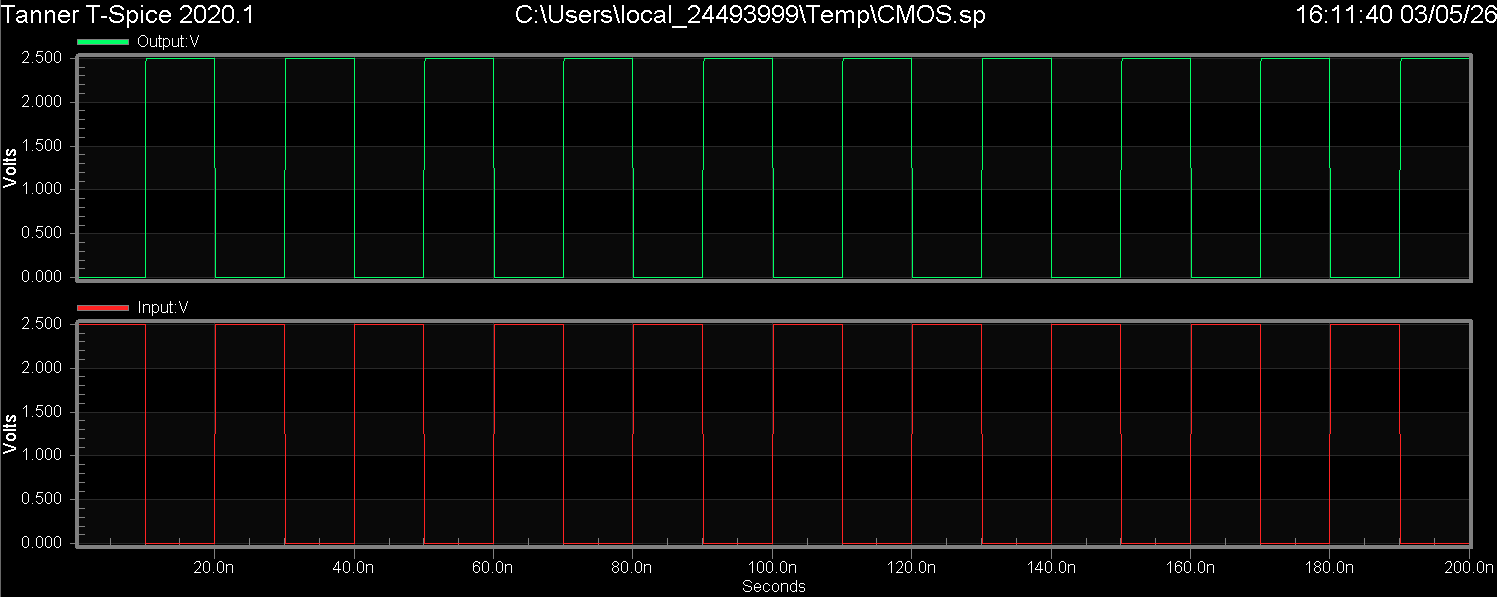
\includegraphics[width=\textwidth]{lab2.1}
    \caption{Transient analysis of the CMOS inverter (Tanner T-Spice, \texttt{CMOS.sp}). Top panel: output voltage (green), 0--2.5\,V. Bottom panel: input voltage (red), 0--2.5\,V. The output is a phase-inverted replica of the input, confirming NOT gate operation.}
    \label{fig:transient}
\end{figure}

\subsection{Rise Time and Fall Time}

Using the SPICE measure components connected to the output node, the timing parameters were extracted from the simulation:

\begin{table}[H]
    \centering
    \caption{Measured rise and fall times at the inverter output.}
    \label{tab:timing}
    \begin{tabular}{lcc}
        \toprule
        \textbf{Parameter}         & \textbf{Measure Name}   & \textbf{Value} \\
        \midrule
        Rise time ($t_r$)          & MeasureRiseTime\_1      & [value]\,ps    \\
        Fall time ($t_f$)          & MeasureFallTime\_1      & [value]\,ps    \\
        \bottomrule
    \end{tabular}
\end{table}

The rise time (output transitioning from 0\,V to $V_{\mathrm{DD}}$, driven by the PMOS) is longer than the fall time (output transitioning from $V_{\mathrm{DD}}$ to 0\,V, driven by the NMOS). This asymmetry is a direct consequence of electron mobility exceeding hole mobility ($\mu_n > \mu_p$) in silicon, meaning the NMOS can discharge the output capacitance more rapidly than the PMOS can charge it.

\subsection{Discussion: Waveforms as Evidence of Inverter Behaviour}

The transient waveforms in Figure~\ref{fig:transient} confirm correct NOT gate operation through the following observations:

\begin{enumerate}
    \item \textbf{Logic inversion:} When $V_{\mathrm{in}}$ is at logic high (2.5\,V), $V_{\mathrm{out}}$ is at logic low (0\,V), and vice versa. The output is at all times the Boolean complement of the input.

    \item \textbf{CMOS switching mechanism:} When $V_{\mathrm{in}}$ is high, Mn1 (NMOS) is ON ($V_{\mathrm{GS,n}} = 2.5$\,V $> V_{\mathrm{Tn}} \approx 0.5$\,V) and Mp1 (PMOS) is OFF ($|V_{\mathrm{GS,p}}| = 0 < |V_{\mathrm{Tp}}|$), pulling the output to GND. When $V_{\mathrm{in}}$ is low, Mp1 is ON and Mn1 is OFF, pulling the output to $V_{\mathrm{DD}}$.

    \item \textbf{Full rail-to-rail swing:} The output transitions fully between 0\,V and 2.5\,V, with no static voltage drop, as expected for CMOS where only one transistor is ON at a time in steady state.

    \item \textbf{No static power dissipation:} In each logic state (input fully high or fully low), one transistor is completely OFF, so there is no DC current path from $V_{\mathrm{DD}}$ to GND and therefore no static power dissipation.

    \item \textbf{Asymmetric transition speeds:} The output rises more slowly than it falls, consistent with $\mu_p < \mu_n$ as discussed above.
\end{enumerate}

%------------------------
%  EXERCISE 2
%------------------------
\section{Exercise 2: Static Analysis of the CMOS Inverter}

\subsection{Circuit Setup}

The transient schematic was modified by replacing the pulsed voltage source with a DC voltage source parameterised as \texttt{VG\_PARA}. A current probe was added at the drain of Mn1 to monitor the drain current $I_{\mathrm{DS}}$. A DC sweep analysis was configured to sweep \texttt{VG\_PARA} from 0\,V to 2.5\,V. Two plots were generated simultaneously: the voltage transfer characteristic ($V_{\mathrm{out}}$ vs $V_{\mathrm{in}}$) and the drain current characteristic ($I_{\mathrm{DS}}$ vs $V_{\mathrm{in}}$).

\subsection{Transfer Characteristic and Power Consumption}

Figure~\ref{fig:static} shows the results of the static analysis.

\begin{figure}[H]
    \centering
    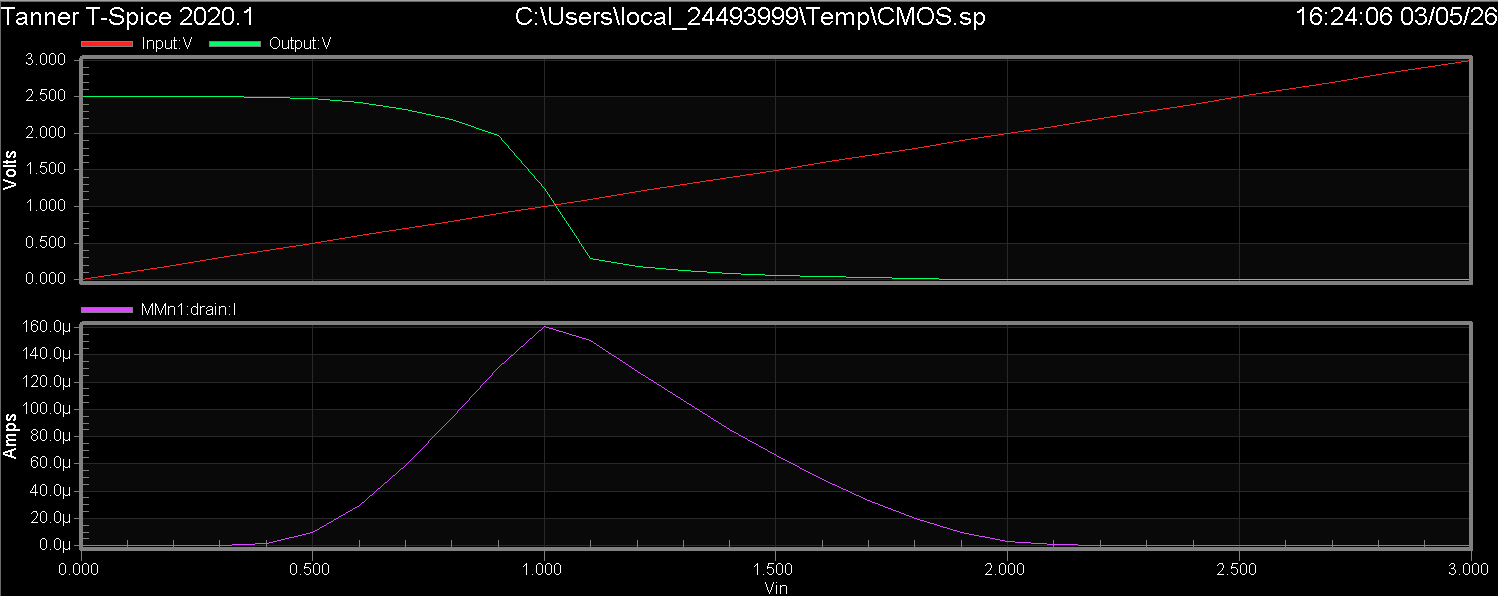
\includegraphics[width=\textwidth]{lab2.2}
    \caption{Static analysis of the CMOS inverter (Tanner T-Spice, \texttt{CMOS.sp}). Top: voltage transfer characteristic (VTC) -- $V_{\mathrm{out}}$ (green) and $V_{\mathrm{in}}$ (red) as functions of $V_{\mathrm{in}}$. Bottom: drain current $I_{\mathrm{DS}}$ (purple) vs $V_{\mathrm{in}}$. The peak of $I_{\mathrm{DS}}$ at approximately $V_{\mathrm{in}} \approx 0.9$\,V ($\approx 160\,\mu$A) marks the point of maximum instantaneous power consumption.}
    \label{fig:static}
\end{figure}

\textbf{Maximum power consumption} occurs at the peak of the $I_{\mathrm{DS}}$ curve, at approximately $V_{\mathrm{in}} \approx 0.9$\,V with a peak current of $\approx 160\,\mu$A. At this point, both the NMOS and PMOS transistors are simultaneously partially conducting, creating a momentary short-circuit (crowbar) current path between $V_{\mathrm{DD}}$ and GND. This crowbar current represents the dominant source of dynamic power dissipation during switching transitions in CMOS logic:
\[
    P_{\mathrm{crowbar}} = I_{\mathrm{DS,peak}} \times V_{\mathrm{DD}} \approx 160\,\mu\mathrm{A} \times 2.5\,\mathrm{V} = 400\,\mu\mathrm{W}
\]
(instantaneous, during the transition). In digital circuits switching at frequency $f$, this contributes to average power proportional to $f$.

\subsection{Skewness of the Transfer Characteristic}

\subsubsection{Observed Threshold}

The VTC in Figure~\ref{fig:static} is visibly skewed to the left. The switching threshold voltage $V_M$ (where $V_{\mathrm{out}} = V_{\mathrm{in}}$) is approximately $V_M \approx 0.9$--$1.0$\,V, which is significantly below the ideal midpoint:
\[
    \frac{V_{\mathrm{DD}}}{2} = \frac{2.5}{2} = 1.25\,\mathrm{V}
\]

\subsubsection{Beta Ratio and Its Role}

The switching threshold of a CMOS inverter is governed by the \textit{Beta ratio}, defined as the ratio of PMOS to NMOS transconductance parameters:
\begin{equation}
    \beta = \frac{\beta_p}{\beta_n} = \frac{\mu_p C_{\mathrm{ox}} (W/L)_p}{\mu_n C_{\mathrm{ox}} (W/L)_n}
    \label{eq:beta}
\end{equation}

Setting $V_{\mathrm{in}} = V_{\mathrm{out}} = V_M$ with both transistors in saturation and equating their drain currents gives the switching threshold:
\begin{equation}
    V_M = \frac{V_{\mathrm{Tn}} + \sqrt{\beta}\,(V_{\mathrm{DD}} - |V_{\mathrm{Tp}}|)}{1 + \sqrt{\beta}}
    \label{eq:VM}
\end{equation}

For $\beta = 1$ and $V_{\mathrm{Tn}} = |V_{\mathrm{Tp}}|$, this simplifies to $V_M = V_{\mathrm{DD}}/2$, as required.

\subsubsection{Beta Ratio Derivation from Lab 1 Data}

From the NMOS output characteristics obtained in Lab 1 (Figure~\ref{fig:nmos_ivds}), in saturation at $V_{\mathrm{GS}} = 2.5$\,V with $V_{\mathrm{Tn}} \approx 0.5$\,V and transistor dimensions $W = 1.5\,\mu\mathrm{m}$, $L = 2\,\mu\mathrm{m}$:

\begin{equation}
    \beta_n = \frac{2\,I_{\mathrm{D,sat}}}{(V_{\mathrm{GS}} - V_{\mathrm{Tn}})^2} = \frac{2 \times 250\,\mu\mathrm{A}}{(2.0\,\mathrm{V})^2} = 125\,\mu\mathrm{A/V}^2
    \label{eq:betan}
\end{equation}

The intrinsic process parameter is then:
\begin{equation}
    \mu_n C_{\mathrm{ox}} = \beta_n \cdot \frac{L}{W} = 125 \times \frac{2}{1.5} \approx 167\,\mu\mathrm{A/V}^2
\end{equation}

\begin{figure}[H]
    \centering
    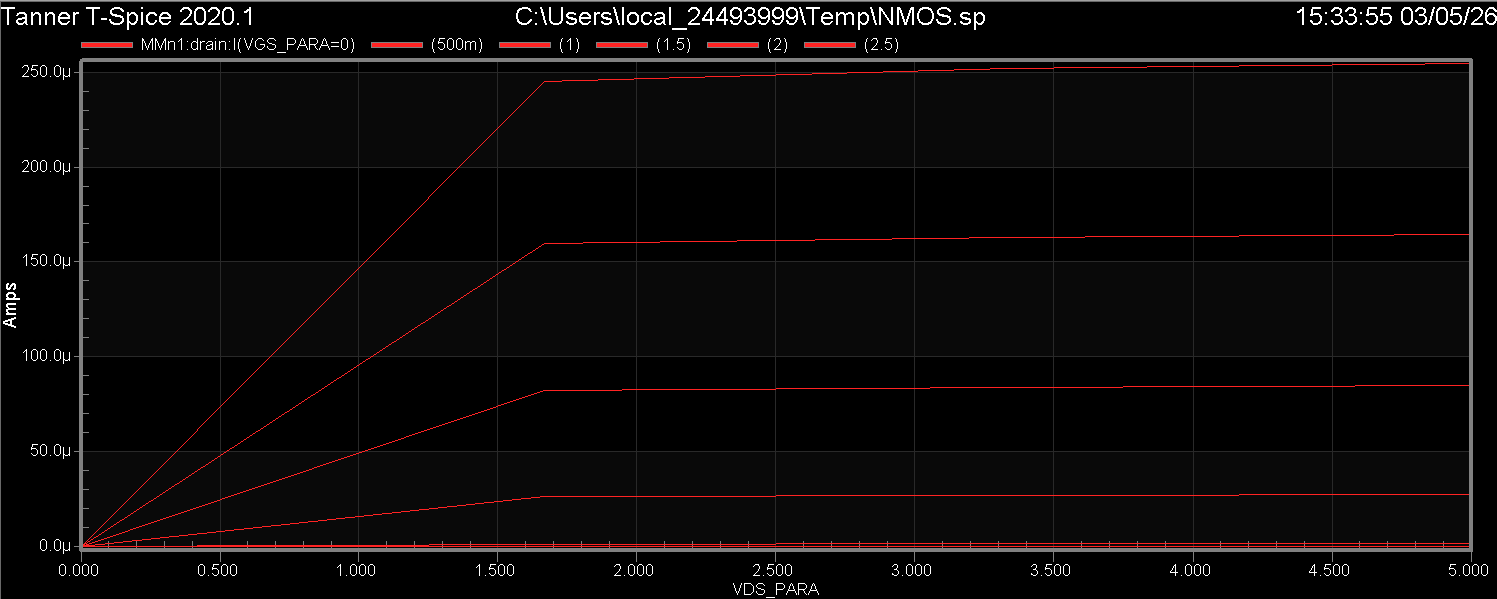
\includegraphics[width=\textwidth]{lab1.2}
    \caption{NMOS25x output characteristics ($I_{\mathrm{DS}}$ vs $V_{\mathrm{DS}}$) from Lab 1, with $V_{\mathrm{GS}}$ stepped from 0\,V to 2.5\,V ($W = 1.5\,\mu\mathrm{m}$, $L = 2\,\mu\mathrm{m}$). At $V_{\mathrm{GS}} = 2.5$\,V (topmost curve), the saturation current is $\approx 250\,\mu$A, giving $\beta_n \approx 125\,\mu\mathrm{A/V}^2$.}
    \label{fig:nmos_ivds}
\end{figure}

For the PMOS25x transistor, hole mobility is lower than electron mobility in the 250\,nm process. From the PMOS $I_{\mathrm{DS}}$ vs $V_{\mathrm{DS}}$ characteristics obtained in Lab 1, the equivalent saturation current at $|V_{\mathrm{GS}}| = 2.5$\,V is substantially lower, corresponding to:
\[
    \frac{\mu_p}{\mu_n} \approx 0.25\text{--}0.4
\]

With the original inverter using identical dimensions for both transistors ($(W/L)_p = (W/L)_n$), the Beta ratio from Equation~\eqref{eq:beta} reduces to:
\begin{equation}
    \beta = \frac{\mu_p C_{\mathrm{ox}}}{\mu_n C_{\mathrm{ox}}} = \frac{\mu_p}{\mu_n} \approx 0.25\text{--}0.4 < 1
\end{equation}

Since $\beta < 1$, the NMOS is the stronger transistor. Substituting into Equation~\eqref{eq:VM} with $\beta \approx 0.25$ (i.e., $\sqrt{\beta} \approx 0.5$), $V_{\mathrm{Tn}} = 0.5$\,V, $|V_{\mathrm{Tp}}| = 0.5$\,V:
\[
    V_M = \frac{0.5 + 0.5 \times (2.5 - 0.5)}{1 + 0.5} = \frac{0.5 + 1.0}{1.5} = 1.0\,\mathrm{V}
\]

This calculated value of $V_M \approx 1.0$\,V is consistent with the observed threshold in the simulation ($\approx 0.9$--$1.0$\,V in Figure~\ref{fig:static}), confirming that the skewed characteristic is caused by the lower hole mobility making the PMOS drive strength less than that of the NMOS with equal dimensions.

\subsection{Correcting the Skewed Characteristic}
\label{sec:correction}

To achieve $V_M = V_{\mathrm{DD}}/2$, the Beta ratio must be unity ($\beta = 1$). Since $C_{\mathrm{ox}}$ and $L$ are fixed, this requires increasing the PMOS width:
\begin{equation}
    \mu_p C_{\mathrm{ox}} \left(\frac{W}{L}\right)_p = \mu_n C_{\mathrm{ox}} \left(\frac{W}{L}\right)_n
    \implies W_p = \frac{\mu_n}{\mu_p} \cdot W_n \approx \frac{1}{0.4} \times 1.5\,\mu\mathrm{m} \approx 3.75\,\mu\mathrm{m}
    \label{eq:Wp_corrected}
\end{equation}

(retaining $L_p = L_n$). The PMOS transistor width was therefore increased to $W_p \approx 3.75\,\mu\mathrm{m}$ in the schematic. Upon re-running the DC sweep, the transfer characteristic became symmetric about $V_{\mathrm{in}} = 1.25$\,V, confirming that the threshold was successfully centred at $V_{\mathrm{DD}}/2$. The peak of the $I_{\mathrm{DS}}$ curve also shifted to the right (towards $V_{\mathrm{in}} \approx 1.25$\,V), as expected for a balanced inverter.

This correction is physically equivalent to compensating for the mobility imbalance ($\mu_n > \mu_p$) by making the PMOS transistor geometrically wider, thereby increasing its effective transconductance to match that of the NMOS.

%------------------------
%  EXERCISE 3
%------------------------
\section{Exercise 3: Inverter Layout using L-Edit}

\subsection{Layout Procedure}

A physical layout of the CMOS inverter was created in L-Edit IC v2020.1 within a new cell in the TannerEDA tutorial library (\texttt{Tutorial.tdb}), using the Generic 250\,nm technology design rules (micron units, major grid 2.5\,$\mu$m, manufacturing grid 5\,nm). The layout was created as a minimum-size implementation, using the shortest permissible wires and transistors to maximise circuit speed and minimise area.

\textbf{PMOS transistor (Part 3):}
\begin{enumerate}
    \item Drew an \textbf{N-Well} layer (box tool) to form the body of the PMOS.
    \item Drew \textbf{P-Implant} within the N-Well to define the source and drain diffusion regions.
    \item Drew an appropriately-sized \textbf{Active} layer over the P-Implant.
    \item Drew a \textbf{Poly} layer across the Active region to form the gate.
    \item Added \textbf{Metal1} and \textbf{Contacts} to connect the source, drain, and gate terminals.
\end{enumerate}

\textbf{NMOS transistor (Part 3):}
\begin{enumerate}
    \item No explicit P-Well was drawn; the empty L-Edit canvas represents the P-substrate (P-well).
    \item Drew \textbf{N-Implant} to define the NMOS source and drain diffusion.
    \item Drew an \textbf{Active} layer over the N-Implant.
    \item Drew \textbf{Poly} across Active for the gate.
    \item Added \textbf{Metal1} and \textbf{Contacts}.
\end{enumerate}

\textbf{Connecting the transistors:}
The Poly layers were extended (Alt + drag) to join the PMOS and NMOS gates, forming the shared \textsc{Input} terminal. The Metal1 layers at the drains of both transistors were extended and connected to form the shared \textsc{Output} node.

\textbf{Supply connections (Part 4):}
\begin{itemize}
    \item \textbf{VDD (PMOS):} A small N-Implant body contact region was placed within the N-Well adjacent to the PMOS, followed by an Active layer, Contact, and Metal1 routed to the PMOS source and labelled \textsc{Vdd}.
    \item \textbf{GND (NMOS):} A small P-Implant body contact was placed in the P-substrate adjacent to the NMOS, followed by an Active layer, Contact, and Metal1 routed to the NMOS source and labelled \textsc{Gnd}.
\end{itemize}

\textbf{Labels (Part 5):} Text labels of 0.5\,$\mu$m size were added using the port tool: \textsc{Input} (Poly layer), \textsc{Output} (Metal1), \textsc{Vdd} (Metal1), \textsc{Gnd} (Metal1).

\subsection{Final Inverter Layout}

Figure~\ref{fig:layout} shows the completed inverter layout with the key terminals identified.

\begin{figure}[H]
    \centering
    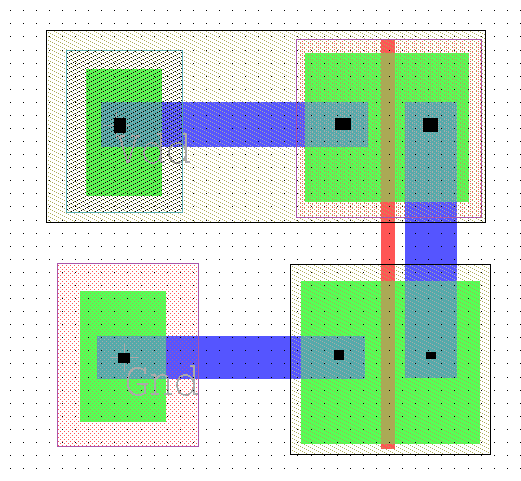
\includegraphics[width=0.72\textwidth]{lab2.3}
    \caption{Completed CMOS inverter layout in L-Edit IC. The PMOS transistor occupies the upper portion, enclosed within the N-well (yellow/dotted border). The NMOS transistor occupies the lower portion in the P-substrate. The vertical red/orange strip is the shared Poly gate (\textsc{Input}). The horizontal blue Metal1 connects the PMOS and NMOS drains (\textsc{Output}). Body contacts for VDD and GND are visible at the left of their respective transistors.}
    \label{fig:layout}
\end{figure}

The terminal assignments are:

\begin{table}[H]
    \centering
    \caption{Terminal identification for the CMOS inverter layout.}
    \label{tab:terminals}
    \begin{tabular}{lllp{7cm}}
        \toprule
        \textbf{Terminal} & \textbf{Transistor} & \textbf{Layer} & \textbf{Description} \\
        \midrule
        Gate (G)     & PMOS \& NMOS & Poly   & Shared gate (vertical strip) --- \textsc{Input} \\
        Drain (D)    & PMOS         & Metal1 & Inner diffusion region, connected to output bus \\
        Drain (D)    & NMOS         & Metal1 & Inner diffusion region, connected to output bus \\
        Source (S)   & PMOS         & Metal1 & Outer diffusion, connected to VDD \\
        Source (S)   & NMOS         & Metal1 & Outer diffusion, connected to GND \\
        Bulk/Body (B)& PMOS         & N-Well & Connected to VDD via N-Implant body contact \\
        Bulk/Body (B)& NMOS         & P-sub  & Connected to GND via P-Implant body contact \\
        \bottomrule
    \end{tabular}
\end{table}

\subsection{Modifying the Layout to Achieve $\beta = 1$}

As derived in Section~\ref{sec:correction}, equalising the Beta ratio requires increasing the PMOS transistor width by a factor of $\mu_n/\mu_p \approx 2.5\times$. In layout terms, this means:

\begin{itemize}
    \item Widening the PMOS channel: extend the N-Well, P-Implant, Active, and Metal1 (source and drain) layers in the direction perpendicular to current flow (vertical extension in the standard-cell orientation) from $\approx 1.5\,\mu$m to $\approx 3.75\,\mu$m.
    \item Extending the Poly gate width to span the full new PMOS Active width.
    \item Repositioning or adding additional drain/source contacts to maintain adequate contact density over the wider diffusion region.
    \item The NMOS dimensions remain unchanged.
\end{itemize}

This increases $(W/L)_p$ relative to $(W/L)_n$ by the factor $\mu_n/\mu_p$, making $\beta_p = \beta_n$ and centering the VTC at $V_{\mathrm{DD}}/2$.

\subsection{Alternative CMOS Inverter Layout Topologies}

Standard cell and custom IC design offer several alternative approaches to laying out a CMOS inverter:

\begin{enumerate}
    \item \textbf{Stacked standard cell (used in this lab):} PMOS placed above NMOS with horizontal power rails (VDD at top, GND at bottom) and the shared gate running vertically as Poly. This is the basis of all modern digital standard cell libraries and is highly amenable to automated place-and-route.

    \item \textbf{Folded (interdigitated) layout:} The transistor channel is split into multiple shorter segments (fingers) arranged in parallel. Each finger carries a fraction of the total current. This halves the effective gate width per finger while maintaining the total $W/L$, reducing gate resistance and improving high-frequency performance. Critical for RF and high-speed applications.

    \item \textbf{Abutted cell layout:} Adjacent inverter cells share diffusion regions (source/drain contacts). By abutting cells, the shared diffusion eliminates redundant contacts and metal, significantly reducing layout area in densely packed digital blocks.

    \item \textbf{Differential pair / symmetric layout:} Both PMOS and NMOS are arranged symmetrically around the gate Poly to minimise parasitic imbalances. Used in analog CMOS designs where matching is critical.

    \item \textbf{FinFET layout (sub-22\,nm):} In advanced technology nodes, transistors are three-dimensional FinFETs. The CMOS inverter layout is markedly different: channel width is controlled by the number of fins (discrete steps) rather than a continuous planar width, and the layout resembles a comb structure. Gate length is defined by the fin height.
\end{enumerate}

In modern digital design flows, inverter layouts are automatically generated by synthesis and place-and-route tools using pre-characterised standard cell libraries, with manual layout reserved for custom, analog, or IP-level blocks.

%------------------------
%  CONCLUSION
%------------------------
\section{Conclusion}

This lab demonstrated the full design flow for a CMOS inverter from schematic simulation to physical layout:

\begin{enumerate}
    \item The \textbf{transient analysis} (Exercise 1) confirmed correct NOT gate operation: the output is a full-swing, rail-to-rail logic complement of the input. The measured rise time is longer than the fall time, directly reflecting the mobility asymmetry $\mu_n > \mu_p$ inherent to silicon CMOS technology.

    \item The \textbf{static analysis} (Exercise 2) revealed a skewed voltage transfer characteristic with the switching threshold $V_M \approx 1.0$\,V, below the ideal $V_{\mathrm{DD}}/2 = 1.25$\,V. This was attributed to a Beta ratio $\beta = \mu_p/\mu_n \approx 0.25$--$0.4 < 1$, consistent with the NMOS and PMOS $I_{\mathrm{DS}}$ characteristics from Lab 1. Increasing the PMOS width to $W_p \approx (\mu_n/\mu_p) \times W_n \approx 3.75\,\mu$m corrected the skew, re-centering the threshold at $V_{\mathrm{DD}}/2$. Maximum instantaneous power dissipation occurs at the switching threshold, where both transistors partially conduct simultaneously.

    \item The \textbf{L-Edit layout} (Exercise 3) implemented the CMOS inverter at the physical design level using the Generic 250\,nm layer stack (N-Well, P-Implant, N-Implant, Active, Poly, Metal1, Contacts). Achieving $\beta = 1$ in the layout requires widening the PMOS active region by $\sim$2.5$\times$ relative to the NMOS while keeping the channel lengths equal.
\end{enumerate}

\end{document}
